\documentclass{standalone}
\usepackage[scaled=0.95]{helvet}  % Load Helvetica font, slightly scaled for better appearance
\usepackage[T1]{fontenc}         % Ensure proper font encoding
\renewcommand{\familydefault}{\sfdefault}  % Set Helvetica as the default font

\usepackage{tikz}
\usetikzlibrary{positioning, er, fit}



\begin{document}

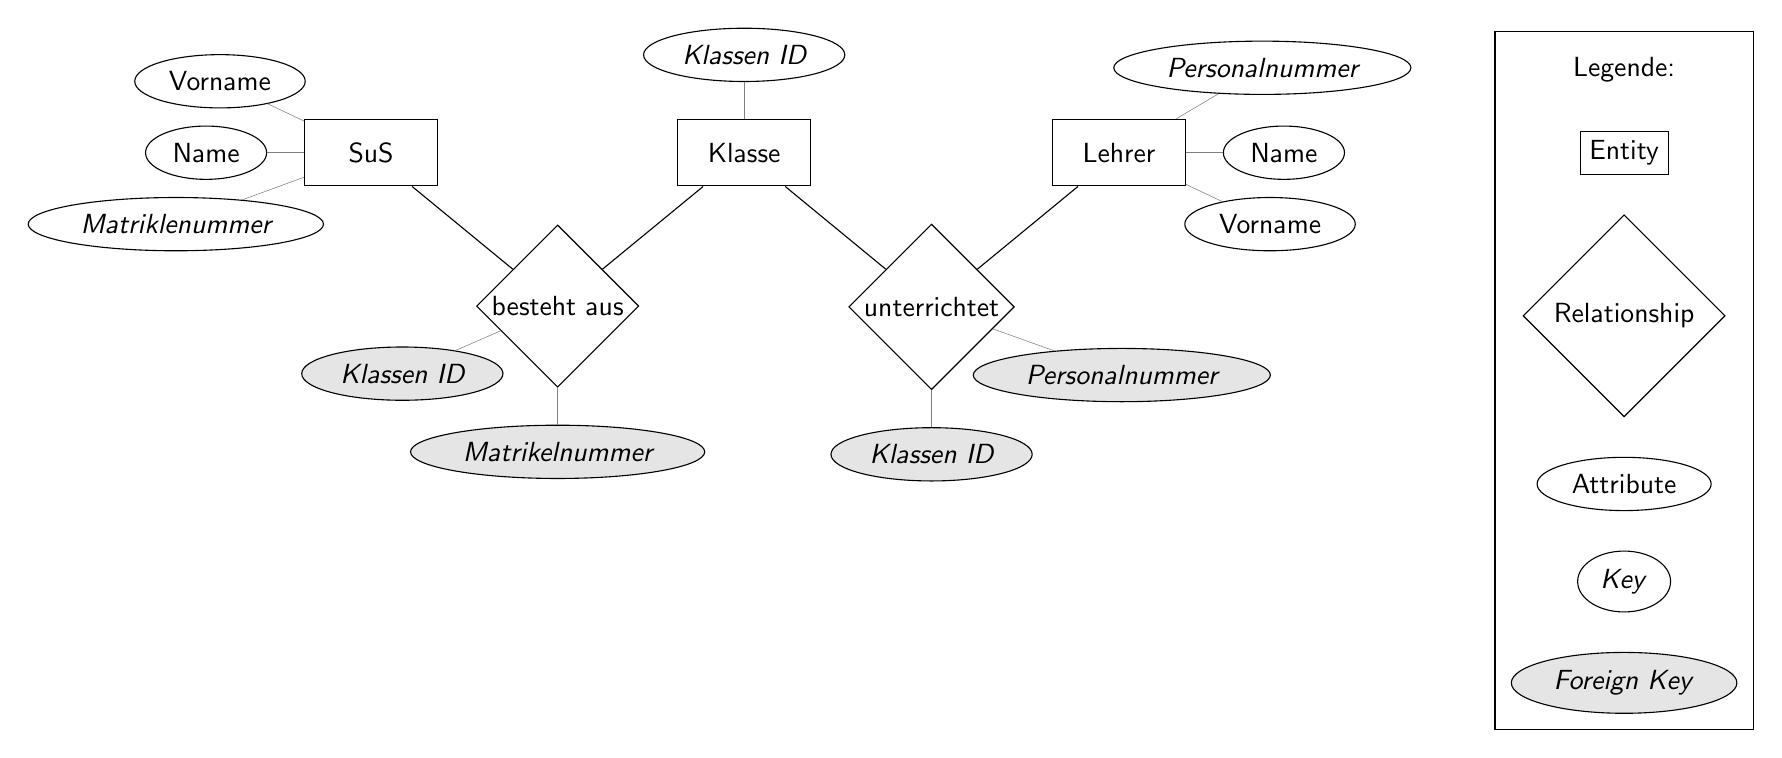
\begin{tikzpicture}
    \node[entity, 
          pin={[key attribute]210:Matriklenummer},
          pin={[attribute]180:Name},
          pin={[attribute]150:Vorname}] (sus) {SuS};
    \node[relationship, below right =of sus,
          pin={[key attribute, fill=gray!20]210:Klassen ID},
          pin={[key attribute, fill=gray!20]270:Matrikelnummer}] (ba) {besteht aus};
    \node[entity, above right =of ba,
          pin={[key attribute]90:Klassen ID}] (kl) {Klasse};
    \node[relationship, below right =of kl,
          pin={[key attribute, fill=gray!20]270:Klassen ID},
          pin={[key attribute, fill=gray!20]330:Personalnummer}] (u) {unterrichtet};
    \node[entity, above right =of u,
          pin={[key attribute]60:Personalnummer},
          pin={[attribute]0:Name},
          pin={[attribute]330:Vorname}] (le) {Lehrer};

    \draw (sus) -- (ba);
    \draw (ba) -- (kl);
    \draw (kl) -- (u);
    \draw (u) -- (le);

    \node[draw, rectangle, right=5cm of le] (entity) {Entity};
    \node[draw, diamond, below = 0.5cm of entity] (relationship) {Relationship};
    \node[draw, ellipse, below = 0.5cm of relationship] (attribute) {Attribute};
    \node[draw, ellipse, below = 0.5cm of attribute] (key) {\textit{Key}};
    \node[draw, ellipse, fill=gray!20, below = 0.5cm of key] (fk)
    {\textit{Foreign Key}};
    \node[above = 0.5cm of entity] (legend) {Legende:};
    \node[draw, fit=(legend)(entity)(relationship)(attribute)(key)(fk), 
          inner sep=0.2cm] (legendbox) {};
\end{tikzpicture}
\end{document}